%clase del documento
\documentclass[a4paper,12pt]{book}

%paquete de idioma y codificación de caracteres
\usepackage[spanish]{babel}
\usepackage[utf8]{inputenc}
\usepackage{afterpage}

%figuras en un lugar determinado
\usepackage{float}

\usepackage{cite} % para contraer referencias
\usepackage{fancyhdr} % para encabezados y pie de pagina

% soporte gráfico
\usepackage{graphicx} % figuras
\usepackage{subfigure} % subfiguras
\graphicspath{ {images/} }

%indice dentro de secciones
\usepackage{minitoc}

%datos del documento
\author{Ignacio Agüero Salcines}
\title{Especificación Gráfica de Procesos de Recuperación de Datos en LUCA}

\setcounter{tocdepth}{5}
\setcounter{secnumdepth}{5}



\begin{document}
	
	
	\pagestyle{empty}
	\dominitoc% Inicializacion
	\tableofcontents
	\cleardoublepage
	
	\pagestyle{plain}
	
	\listoffigures
	\listoftables
	\thispagestyle{empty}
	\cleardoublepage
	
	\pagenumbering{roman}
	\chapter*{Agradecimientos}
	Me gustaría dar agradecimientos a mi familia y facultad, ya que sin ellos esto no habría sido posible nada de estos.
	
	\vspace{5mm}
	
	\noindent Es importante agradecer también a CIC Consulting Informático por permitirme la oportunidad de realizar el desarrollo del proyecto en su empresa, sin olvidarme de mis compañeros de LUCA, que han sido un gran apoyo durante el mismo..
	
	\vspace{5mm}
	
	\noindent Para finalizar, me gustaría gradecer a mi mentor Pablo, por guiarme durante el desarrollo del proyecto con eficacia y ayudarme a afrontar este trabajo de fin de grado.
	\cleardoublepage
	
	\clearpage
	
	\chapter*{Resumen}
	Las empresas actuales no utilizan un único sistema de información que de soporte a sus procesos de trabajo, sino un  ecosistema de sistemas información que dan soporte a diferentes procesos de negocio ejecutados dentro de dicha organización. Como consecuencia de esta nueva situación, cuando un usuario	quiere obtener una información concreta cuyos datos residen en varios de estos
	sistemas, necesita acceder a cada uno de estos sistemas, extraer de cada sistema la información que precisa, filtrarla y unificarla para finalmente	obtener los datos requeridos.
	
	\vspace{5mm}
	
	Por ejemplo, una tienda de electrodomésticos podría tener sistemas informáticos diferentes para el departamento de atención al cliente, para el departamento técnico de postventa y para el departamento de compras y adquisiciones.Por tanto, para conocer el estado actual de una reparación, podríamos necesitar:
		\begin{itemize}
			\item  Acceder al primer sistema para obtener el identificador de la incidencia y en qué fase de su gestión se encuentra.
			\item  Comprobado que la incidencia está actualmente en reparación, recuperaríamos otro sistema el estado detallado de la reparación, comprobando que está a la espera de una pieza.
			\item Finalmente accederíamos al sistema de compra y adquisiciones para comprobar cuando está prevista la entrega de dicha pieza. Los sistemas de almacenamiento de la información pueden ser diversos, incluyendo desde un servicio web, una base de datos relacional, un repositorio de ficheros accesible vía FTP o una base de datos NoSQL.
		\end{itemize}
	
	\vspace{5mm}
	
	El objetivo de este proyecto es facilitar dicho proceso de composición al usuario mediante el desarrollo de un mecanismo gráfico para la especificación de estos procesos de composición de consultas.
	

	\vspace{5mm}
	
	\textbf{Palabras clave}: 
	\cleardoublepage
	
	\clearpage
	
	\chapter*{Preface}

	

	\textbf{Keywords}:
	\cleardoublepage
	
	\pagenumbering{arabic}
	\setcounter{page}{1}
	
	\clearpage
	
	\chapter{Introducción}
	
Este primer capítulo describe de forma general la información principal y relevante para poder comprender el funcionamiento del producto actual LUCA, así como los objetivos del proyecto a desarrollar junto con la explicación y motivación del mismo.
	
\section{Introducción}
	
	
En los últimos años, el volumen de datos que una empresa o entidad necesita o es capaz de gestionar o manipular ha aumentado de forma vertiginosa. Estos datos se almacenan en fuentes de diversos tipos, abarcando elementos tan dispares como bases de datos relacionales, hojas XML o repositorios FTP, a los cuales se accede mediante diferentes formas y lenguajes. Por tanto, un nuevo problema que debemos enfrentar, adicional al del volumen de datos a manipular, es que para acceder cierta información es necesario muchas veces establecer comunicaciones entre diferentes fuentes.

\vspace{5mm}
			
%%===================================================================%%
%% NOTE(Pablo): Meter aquí el ejemplo del resumen de nuevo, si se
%%              quiere más detallado
%%===================================================================%%

%% Init resumen

	 Como consecuencia de esta nueva situación, cuando un usuario	quiere obtener una información concreta cuyos datos residen en varios de estos
sistemas, necesita acceder a cada uno de estos sistemas, extraer de cada sistema la información que precisa, filtrarla y unificarla para finalmente	obtener los datos requeridos.

\vspace{5mm}

Por ejemplo, una tienda de electrodomésticos podría tener sistemas informáticos diferentes para el departamento de atención al cliente, para el departamento técnico de postventa y para el departamento de compras y adquisiciones.Por tanto, para conocer el estado actual de una reparación, podríamos necesitar:
\begin{itemize}
	\item  Acceder al primer sistema para obtener el identificador de la incidencia y en qué fase de su gestión se encuentra.
	\item  Comprobado que la incidencia está actualmente en reparación, recuperaríamos otro sistema el estado detallado de la reparación, comprobando que está a la espera de una pieza.
	\item Finalmente accederíamos al sistema de compra y adquisiciones para comprobar cuando está prevista la entrega de dicha pieza. Los sistemas de almacenamiento de la información pueden ser diversos, incluyendo desde un servicio web, una base de datos relacional, un repositorio de ficheros accesible vía FTP o una base de datos NoSQL.
\end{itemize}


\section{LUCA}

%% End resumen
			
Con el objetivo de facilitar este proceso de recuperación de información almacenada en sistemas y fuentes de datos hetereogéneas, dentro de la empresa CIC, se está desarrollando una aplicación denominada LUCA. Para facilitar este proceso de recuperación de información, LUCA proporciona un lenguaje común para todas las fuentes de datos a unificar, permitiendo al usuario abstraerse de los detalles de cada fuente.

\vspace{5mm}

%%===================================================================%%
%% NOTE(Pablo): Poner un ejemplo sencillo que muestre el
%%              funcionamiento de LUCA
%%===================================================================%%



%% Ejemplo Luca

A continuación se explica brevemente el funcionamiento de Luca con algunos ejemplo gráficos orientativos para ayudar a la comprensión del propio funcionamiento.

\vspace{5mm}

Para explicar el funcionamiento principal de dicho producto, se pretende describir el proceso de creación y ejecución de una consulta a un servicio REST.

\vspace{5mm}

En la vista inicial nos encontramos con una lista de consultas ya almacenadas, así como, una serie de filtros y opciones para la creación, ejecución y edición de consultas. Como se pretende explicar la creación y ejecución de una consulta, para avanzar en la vista se seleccionaría la creación de una nueva consulta.


\vspace{5mm}

A continuación, se muestra un ejemplo sobre un servicio REST, concretamente sobre el servicio REST de información de la flota de autobuses de Santander (TUS), donde tras introducir el identificador de una parada de autobús, se devolverá la información relativa a dicha parada, como es la localización.


	
	\begin{figure}[H]
		\centering
 		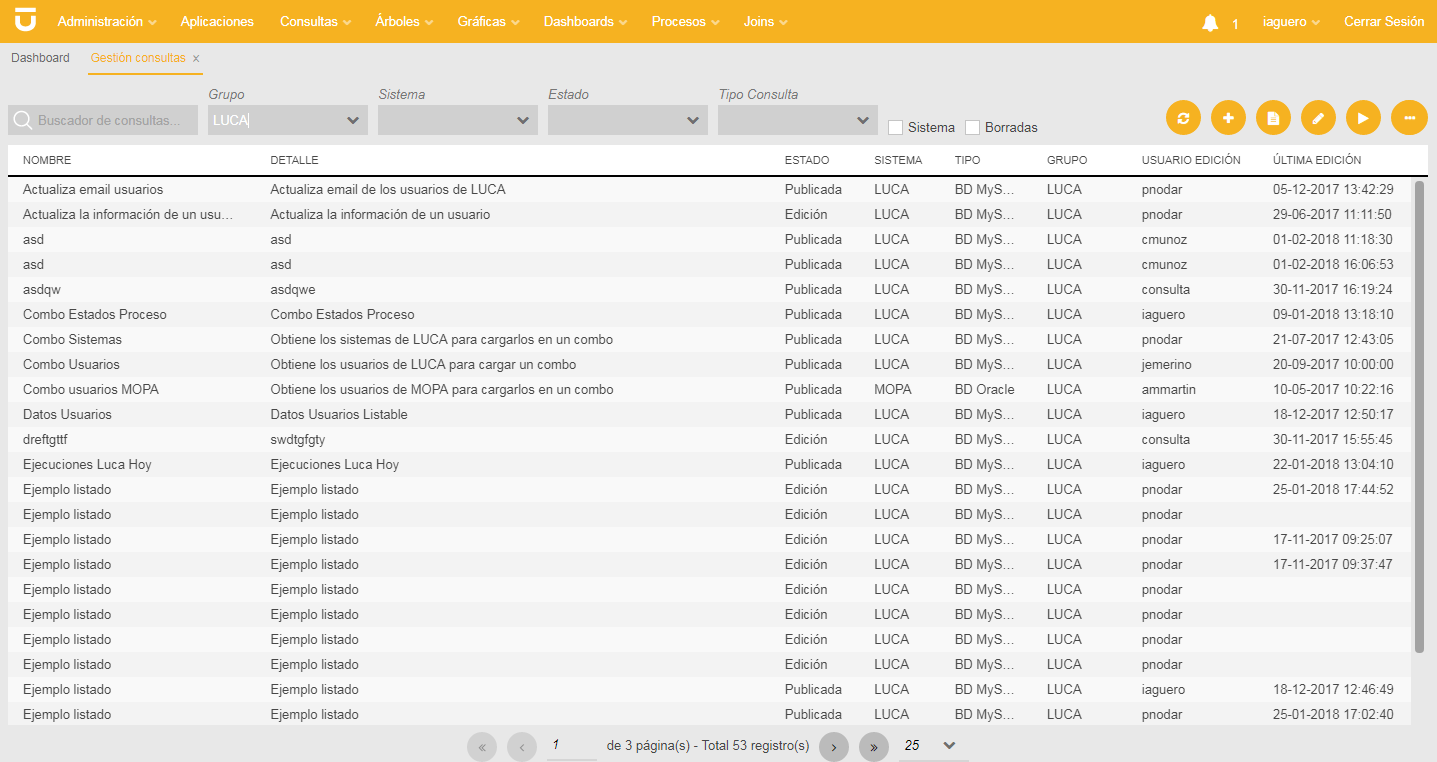
\includegraphics[scale=0.5]{capturasLuca/gestionConsultas.png}
		\caption{Vista de Gestión de Consultas}\label{fig:gestionConsulta}
	\end{figure}

Tras seleccionar la opción de creación de una nueva consulta, se muestra una vista en la que se permite agregar toda la información relativa a la consulta, como son las variables de entrada o de salida, o el tipo de salida que se desea recibir.

\vspace{5mm}

Una vez introducido el identificador de la parada, y seleccionado el botón de ejecución para llevar a cabo la ejecución de la consulta, se muestra el resultado de la consulta, el cuál puede ser visualizado de diferentes formas en función del recurso al que se llama.


	\begin{figure}[H]
		\centering
		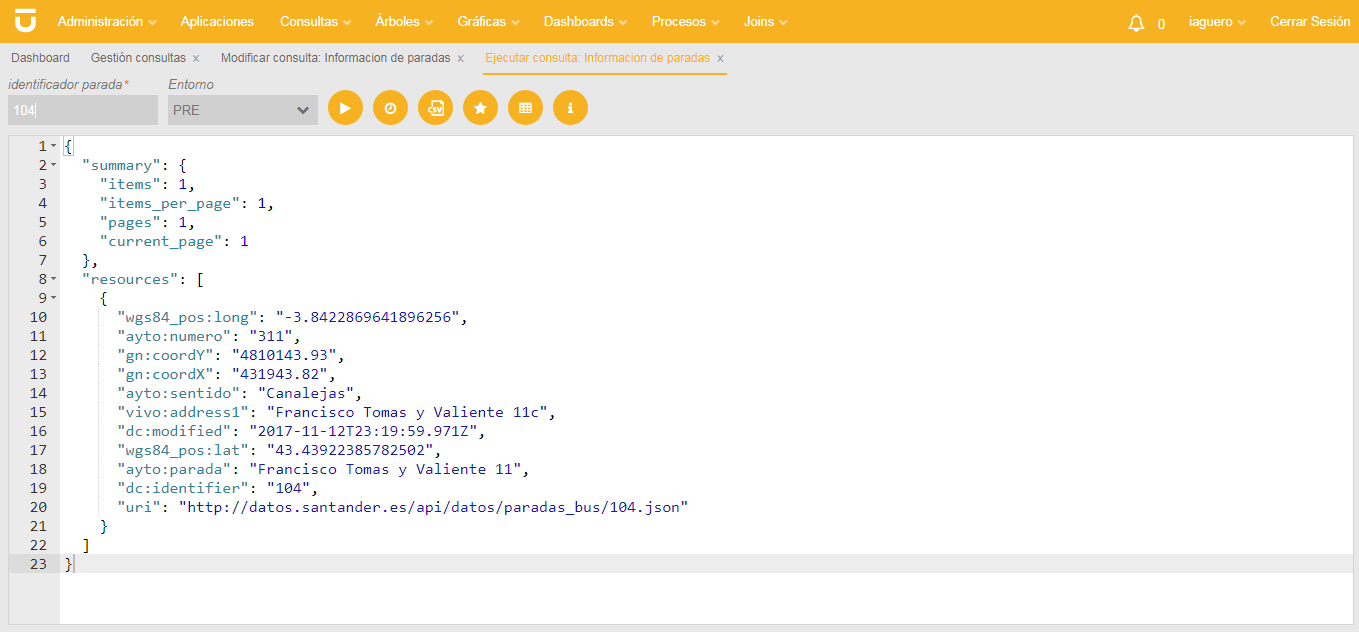
\includegraphics[scale=0.5]{capturasLuca/ejecucionConsulta.png}
		\caption{Vista de Ejecución de Consultas}\label{fig:ejecucionConsultas}
	\end{figure}


\vspace{5mm}


%% Fin ejemplo Luca

Actualmente LUCA proporciona mecanismos para permitir al usuario recuperar de manera uniforme información de diferentes fuentes de datos. No obstante, LUCA actualmente sólo es capaz recuperar información de una única fuente de datos a la vez. Por tanto, cuando es necesario combinar información procedente de distintas fuentes, el propio usuario es el que debe realizar dicho proceso de composición, ejecutando cada consulta a mano, y utilizando las salidas de cada una de ellas como las entradas de las siguientes.

\vspace{5mm}
			
%%===================================================================%%
%% NOTE(Pablo): Poner un ejemplo cómo es el proceso de composición
%%              a mano
%%===================================================================%%

Un ejemplo de dicho proceso de composición sería la necesidad de un dependiente de una tienda de electrodomésticos de obtener la edad de los usuarios que compraron lavadoras durante el mes pasado. Actualmente, los pasos o consecución de consultas que debería de realizar serían las siguientes:

\begin{itemize}
	\item  Primero necesitaría obtener el registro de compras del mes pasado del sistema.
	\item  Después, tras apuntarse dicho registro, tendría que, uno por uno, seleccionar los que se corresponden con lavadoras.
	\item Una vez que el usuario tiene las lavadoras compradas el mes pasado, éste tendría que recoger que usuarios han comprado las lavadoras.
	\item Por último, el usuario debería de buscar en el sistema cada usuario que ha realizado la compra, con el nombre obtenido previamente.
\end{itemize}

Se puede observar que el usuario tiene un engorroso desarrollo de acciones para poder obtener el resultado deseado.

\vspace{5mm}

%% Fin ejemplo composición

El objetivo de este proyecto es facilitar dicho proceso de composición al usuario mediante el desarrollo de un mecanismo gráfico para la especificación de estos procesos de composición de consultas.

\vspace{5mm}

%%===================================================================%%
%% NOTE(Pablo): Dar algunos detalles técnicos de cómo se pretente
%%              construir esto.
%%===================================================================%%
Para llevar a cabo esta tarea, se pretende realizar un sistema que permita visualmente utilizar las consultas ya almacenadas, para posteriormente relacionarlas entre sí mediante sus entradas y salidas y los tipos de las mismas. De esta forma, se podrá ejecutar automáticamente una cadena de consultas para obtener un resultado concreto, bajo un único concepto llamado Proceso.


\section{Ingeniería de Requisitos}

En esta sección se contará el proceso llevado a cabo para aprender o entender la estructuración y definición de requisitos de la actual LUCA, así como la propia descripción de los requisitos que serán necesarios para la implementación del proyecto a realizar.

\subsection{Proceso de integración en LUCA}

El primer paso llevado a cabo para la introducción en el producto de LUCA y entender así su funcionamiento, fue una reunión con el Jefe de Proyecto y con el Gerente para describir, analizar y explicar todos los aspectos de LUCA.

\subsection{Definición de Requisitos}

Una vez aclarados los términos del actual LUCA, se abordo el incremento que se quería llevar a cabo, del que parte este Trabajo de Fin de Grado. Se explicaron los términos de Proceso, variables de entradas y de salidas, consultas y demás.

\vspace{5mm}

Además de la explicación, se proporcionaron unos documentos técnicos tanto del componente gráfico del proceso como del incremento sobre LUCA. Estos documentos pueden encontrarse en el Anexo adjunto a la memoria.

\vspace{5mm}

Como ya se ha mencionado, en estos documentos se pueden encontrar los requisitos técnicos atribuidos al proyecto, pero, de forma resumida, se centran en tres pilares:

\begin{itemize}
	\item  Concatenación de las consultas entre si pertenecientes a un mismo proceso.
	\item  Visualización del progreso de ejecución del proceso.
	\item Aplicar criterios de navegación a partir de los resultados de salidas.
\end{itemize}

La especificación de estos requisitos se encuentra en los documentos técnicos citados anteriormente.


	 
	
	\clearpage
	
	\chapter{Antecedentes}

\minitoc
	
\section{Go.JS}

Go.JS~\cite{gojs} es una biblioteca de JavaScript para implementar editores gráficos dentro de interfaces web. GoJS facilita la implementación de tareas tales como definición de símbolos gráficos, gestión de paletas de símbolos, arrastrar y soltar (\emph{drag and drop}), copiar y pegar, edición de etiquetas de texto asociadas a símbolos gráficos, menús contextuales, función de deshacer o la gestión de eventos de ratón, entre muchos otros elementos.

Para ilustrar el funcionamiento de GoJS, a continuación se mostrará a modeo de ejemplo cómo crear un editor gráfico para diseñar unos pseudo diagramas de flujo compuestos por círculos y rectángulos interconectados por flechas. Dicho editor se muestra en la Figura~\ref{fig:gojssample}.

\begin{figure}[!tb]
	\centering
	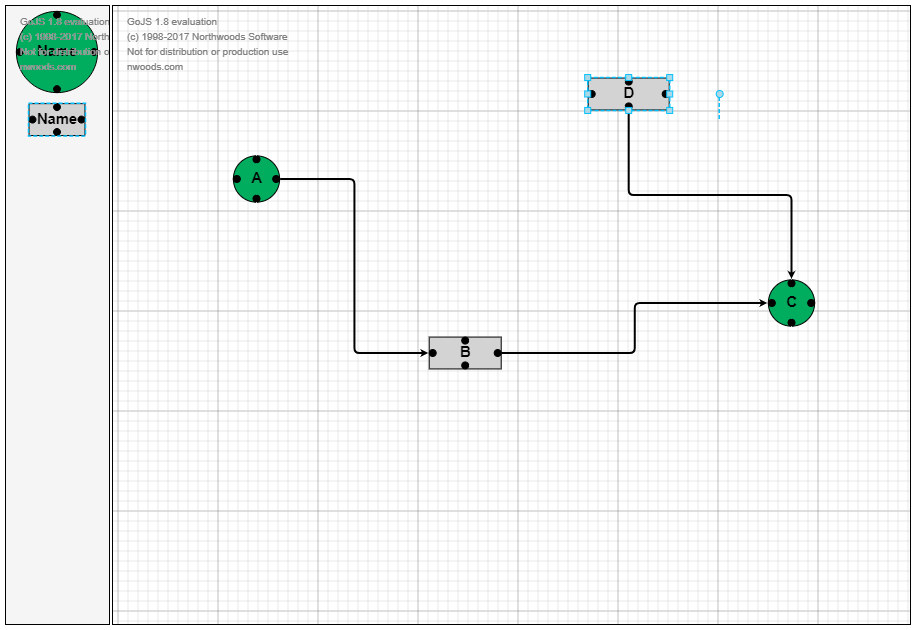
\includegraphics[width=\linewidth]{gojssample.png}
	\caption{Editor gráfico creado en GoJS}
    \label{fig:gojssample}
\end{figure}

Para comenzar, cabe destacar que, es necesario reservar dos secciones de la página HTML que lo contiene. Una sección albergará la paleta con los elementos gráficos del editor, que en este caso serán sólo el círculo y el rectángulo, y otra sección para el diagrama o lienzo sobre el que se depositarán los elementos gráficos.

A continuación, se debe realizar una serie de acciones a nivel de Javascript para proporcionar tanto a la paleta de dibujo como al área de dibujo del comportamiento deseado. En primer lugar, crearemos una variable \texttt{\$} que dé acceso al entorno GoJS. Esto se realiza mediante la llamada a la sentencia \texttt{make} de librería \emph{GraphObject} de GoJS (Figura~\ref{fig:asignacionDollar}, Línea~1).

\begin{figure}[!tb]
	\centering
	\begin{lstlisting}[language=JavaScript]
	var $ = go.GraphObject.make;\end{lstlisting}
	\caption{Asignación de la variable \texttt{\$}}
	\label{fig:asignacionDollar}
\end{figure}

Seguidamente, se personaliza la sección HTML reservada al diagrama, denominada \texttt{myDiagramDiv} (Figura~\ref{fig:creacionDiagrama}, Líneas~01-13), asignándole un \emph{grid} o cuadrícula de fondo (Figura~\ref{fig:creacionDiagrama}, Líneas~04-09), especificando los colores de las líneas de la cuadrícula (mediante la propiedad \emph{stroke}) y dándole la capacidad de poder arrastrar elementos sobre él (Figura~\ref{fig:creacionDiagrama}, Línea~10).

\begin{figure}[!tb]
	\centering
	\begin{lstlisting}[language=JavaScript]
	myDiagram =
		$(go.Diagram, "myDiagramDiv",
		{
			grid: $(go.Panel, "Grid",
				$(go.Shape, "LineH", { stroke: "lightgray", strokeWidth: 0.5 }),
				$(go.Shape, "LineH", { stroke: "gray", strokeWidth: 0.5, interval: 10 }),
				$(go.Shape, "LineV", { stroke: "lightgray", strokeWidth: 0.5 }),
				$(go.Shape, "LineV", { stroke: "gray", strokeWidth: 0.5, interval: 10 })
			),
			allowDrop: true,
		}
	);\end{lstlisting}
	\caption{Creación de un diagrama en GoJS}
	\label{fig:creacionDiagrama}
\end{figure}

A continuación deberemos definir lo que en GoJS se conoce como la \emph{plantilla de nodos} o \emph{node template}. Esta plantilla define el comportamiento genérico de todos los nodos que compondrán nuestro diagrama. Estos nodos, en nuestro caso, serán rectángulos y círculos. La Figura~\ref{fig:patronNodo} muestra cómo se crea el patrón que servirán de esqueleto para todos los nodos de nuestro diagrama. 

\begin{figure}[!tb]
	\centering
	\begin{lstlisting}[language=JavaScript]
	myDiagram.nodeTemplate =
		$(go.Node, "Spot",
		{ 
			locationSpot: go.Spot.Center 
		},
		new go.Binding("location").makeTwoWay(go.Point.stringify),
		{ 
			selectable: true, 
			selectionAdornmentTemplate: nodeSelectionAdornment 
		},
		{ 
			resizable: true, 
			resizeObjectName: "PANEL", 
			resizeAdornmentTemplate: nodeResizeAdornment 
		},
		{ 
			rotatable: true, 
			rotateAdornmentTemplate: nodeRotateAdornment 
		},
	
		$(go.Panel, "Auto",
		{ 
			name: "PANEL" 
		},
		$(go.Shape,
		{
			portId: "",
			fromLinkable: true, toLinkable: true, cursor: "pointer",
		},
		new go.Binding("figure"),
		new go.Binding("fill")),
		$(go.TextBlock,
		{
			maxSize: new go.Size(50, 50),
			editable: true
		},
		new go.Binding("text").makeTwoWay())
		)
	);\end{lstlisting}
\caption{Declaración del patrón del Nodo}
\label{fig:patronNodo}
\end{figure}

Para crear la definición un nodo lo primero es declarar el nodo con \texttt{\$(go.Node} (Figura~\ref{fig:patronNodo},~Línea~2).
A continuación, especificamos, mediante la definición de ciertas propiedades, cómo se comportará el nodo (Figura~\ref{fig:patronNodo}, Líneas~5-24). En nuestro caso, se indica que los nodo, con carácter general, podrán ser seleccionados, redimensionados y rotados (Figura~\ref{fig:patronNodo}, Líneas~7-19, respectivamente). Se establece que los nodos aparecerán localizados por defecto en el centro del diagrama en el momento de su creación (Figura~\ref{fig:patronNodo}, Línea~4).
Además, se indica que la propiedad \texttt{location}, que establece la posición del nodo, queda expuesta para su modificación desde el exterior (Figura~\ref{fig:patronNodo}, Línea~04).

Siempre que se crea un nodo, se reserva un espacio sobre el que se van a situar los diferentes elementos del nodo. En nuestro ejemplo, este espacio recibe el nombre de \emph{panel}(Figura~\ref{fig:patronNodo}, Línea~21). El panel actúa como contenedor de la figura (\emph{shape}) (Figura~\ref{fig:patronNodo}, Línea~25), que es la encargada de definir la forma del nodo. En nuestro caso, dicho panel podrá poseer diferentes formas (como serán el circulo y el rectángulo) y colores gracias a los \emph{bindings}, que son los que hacen que estas propiedades sean modificables programáticamente (Figura~\ref{fig:patronNodo}, Líneas~30-31). Además, cada nodo poseerá un identificador propio, denominado \emph{portId} (Figura~\ref{fig:patronNodo}, Línea~27) y todos los nodos pueden recibir conexiones tanto de entrado como de salida (\emph{toLinkable} y \texttt{fromLinkable}) (Figura~\ref{fig:patronNodo}, Línea~28). Por último, cada nodo poseerá una etiqueta de texto que permitirá especificar su nombre, el cual también puede ser modificado externamente (Figura~\ref{fig:patronNodo}, Líneas~32-38).

Una vez definidas las propiedades básicas de un nodo, el siguiente paso es definir cómo enlazar dichos nodos. Para ello debemos definir dos elementos: \emph{puertos} y \emph{enlaces}. Los enlaces son los elementos que permiten conectar nodos, y los puertos de un nodo son los puntos de dicho nodo desde donde puede partir un enlace o a dónde puede llegar un enlace.  En la Figura~\ref{fig:gojssample}, estos puertos aparecen aparecen como unos círculos negros en los extremos de las figuras.

\begin{figure}[!tb]
	\centering
	\begin{lstlisting}[language=JavaScript]
	function makePort(name, spot) {
		return $(go.Shape, "Circle",
		{
			desiredSize: new go.Size(7, 7),
			alignment: spot,
			alignmentFocus: spot,
			portId: name,
			fromLinkable: true, toLinkable: true,
			cursor: "pointer"
		});
	}\end{lstlisting}
	\caption{Función MakePort}
	\label{fig:funcionMakeport}
\end{figure}
	
Para añadir puertos a los nodos se ha creado una función una función llamada \emph{makePort}, la cual se muestra en la Figura~\ref{fig:funcionMakeport}. Este fragmento de código define un puerto como una forma circular con un identificador (Figura~\ref{fig:funcionMakeport}, Línea~07), una posición (Figura~\ref{fig:funcionMakeport}, Líneas~05-06) y un tamaño (Figura~\ref{fig:funcionMakeport}, Línea~04). Finalmente, usando esta función, añadimos cuatro llamadas a a misma al final de la plantilla de nodos, con el objeto de crear un puerto a cada lado del eje de cada nodo (Figura~\ref{fig:patronNodoFinal}, Línea~04).

\begin{figure}[!tb]
	\centering
	\begin{lstlisting}[language=JavaScript]
	myDiagram.nodeTemplate =
		$(go.Node, "Spot",
		{ locationSpot: go.Spot.Center },
        ...
		makePort("T", go.Spot.Top),
		makePort("L", go.Spot.Left),
		makePort("R", go.Spot.Right),
		makePort("B", go.Spot.Bottom)
	);\end{lstlisting}
	\caption{Patrón Nodo con Puertos}
	\label{fig:patronNodoFinal}
\end{figure}

Una vez definidos los puertos, especificamos cómo se comportarán los enlaces entre nodos (Figura~\ref{fig:patronlink}). En nuestro caso, se declara que los enlaces irán de un nodo principal \texttt{isPanelMain} a uno secundario,  se efine el grosor del enlace y se establece que el enlace poseerá una flecha al final del mismo (\emph{toArrow: "Standard"}).

\begin{figure}[!tb]
	\centering
	\begin{lstlisting}[language=JavaScript]
	myDiagram.linkTemplate =
		$(go.Link,
			$(go.Shape,
			{ isPanelMain: true, strokeWidth: 2 }),
			$(go.Shape,
			{ toArrow: "Standard", stroke: null }
		)
	)\end{lstlisting}
\caption{Declaración del patrón del Link}
\label{fig:patronlink}
\end{figure}


\begin{figure}[!tb]
	\centering
\begin{lstlisting}[language=JavaScript]
myPalette =
	$(go.Palette, "myPaletteDiv",
	{
		nodeTemplateMap: myDiagram.nodeTemplateMap,
		model: new go.GraphLinksModel([
			{ 
				text: "Name", 
				figure: "Circle", 
				fill: "#00AD5F" 
			},
			{ 
				text: "Name", 
				figure: "Rectangle", 
				fill: "lightgray" 
			}
			])
		}
);\end{lstlisting}
\caption{Creación de la Paleta de Nodos}
\label{fig:paletaNodos}
\end{figure}

Por último, se procede a crear la paleta que contendrá los círculos y los rectángulos, tal como se muestra en la Figura~\ref{fig:paletaNodos}. Como se puede observar, la paleta se sitúa sobre una sección HTML denominada \emph{myPalleteDiv} (Figura~\ref{fig:paletaNodos}, Línea~XX), la cual fue reservada con anterioridad. Para la definición de los nodos que estarán dentro de la paleta se utiliza el mismo patrón e nodos creado con anterioridad (Figura~\ref{fig:paletaNodos}). Finalmente, por último, se declara el \emph{modelo}, que es el conjunto de figuras concretas que poseerá dicha paleta. Para crear los elementos del modelo, se instancia la plantilla de nodos y se cambian sus propiedades con objeto de crear objetos diferentes. En nuestro caso, creamos círculo de color verde (Figura~\ref{fig:paletaNodos}, Línea~06) y rectángulos de color gris (Figura~\ref{fig:paletaNodos}, Línea~07), ambos con \texttt{Name} como nombre por defecto, el cual podrá ser luego editado.

Una vez definidos estos elementos, nuestro editor gráfico queda implementado, y GoJS se encargará de dibujar la paleta y el diagrama, así como, de pintar los elementos sobre el área de dibujo cuando éstos sean seleccionados en la paleta, permitiendo arrastrarlos, redimensionarlos o renombrarlos, entre otras funciones.

\section{Patrón \emph{Model-View-Presenter (MVP)}}

%% Detallar aquí brevemente y con claridad, a ser posible, utilizando una figura
%% para ello, el funcionamiento del patrón MVP.
\begin{figure}[H]
	\centering
	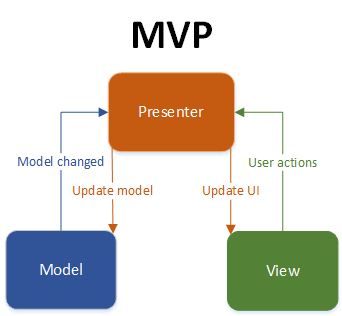
\includegraphics[width=0.6\linewidth]{mvp.png}
	\caption{Patrón Modelo-Vista-Presentador}\label{fig:mvp}
\end{figure}

Este patrón esta orientado a crear interfaces de usuario y su objetivo es separar la lógica de la aplicación de los detalles estéticos de la interfaz. Se compone de tres módulos independientes: \emph{modelo}, \emph{vista} y \emph{presentador} (ver Figura~\ref{fig:mvp}).

%% Poner Figura  


El \emph{modelo} es el encargado de gestionar los datos de la aplicación, y que de alguna forma serán mostrados al usuario. La \emph{vista} es una interfaz de usuario, normalmente gráfica, que se encarga de mostrar datos al usuario de la manera más amigable posible. Por último el presentador se sitúa entre el \emph{Modelo} y la \emph{Vista} y se encarga de conectar ambos elementos. Los eventos realizados sobre la interfaz de usuario se delegan en el presentador, que es el que decide qué cambios se deberán realizar sobre la interfaz gráfica. Para ello puede acceder a datos al modelo, o solicitar la modificación de los mismos. 

De esta forma se separa lo que es la lógica de navegación y procesamiento de eventos de los detalles de cómo se organiza exactamente una interfaz de usuario. De este modo, se aisla dicha lógica de cambios estéticos que pudiesen producrise en dicha interfaz. 

La siguiente sección mostrará como \emph{Vaadin}, un framework para el desarrollo de aplicaciones web, implementa de una manera concreta este patrón.

 



\label{sec:mvp} 

\section{Vaadin}
 		


\emph{Vaadin}~\cite{vaadin} es un \textbf{framework} para el desarrollo de aplicaciones \emph{web} avanzadas, también conocidas como \emph{Rich-Internet Applications (RIA)}~\cite{ria}. El objetivo del paradigma \emph{RIA} es desarrollar aplicaciones \emph{web} con interfaces avanzadas que les haga asemejarse a las aplicaciones de escritorio. La principal ventaja que aporta \emph{Vaadin} es que permite escribir aplicaciones en código Java, como si fuesen de escritorio, y luego este código es transformado para que funcione en tecnologías web como HTML (HyperText Markup Language)~\cite{html}, CSS (Cascading Style Sheets)~\cite{css}, Javascript~\cite{javascript}, HTTP (Hypertext Transfer Protocol)~\cite{http} o AJAX (Asynchronous JavaScript and XML)~\cite{ajax}.

Una de las características diferenciadores de \texttt{Vaadin} es que, al contrario de las librerías de JavaScript tradicionales, \emph{Vaadin} también contempla la parte del servidor, por lo se generan tanto las llamadas al servidor desde la interfaz gráfica (\emph{front-end}) como la recepción y tratamiento de esas llamadas en la parte del servidor (\emph{back-end}).



 	
 \subsection{Ejemplo Vaadin}
 	
\begin{figure}[!tb]
	\centering
	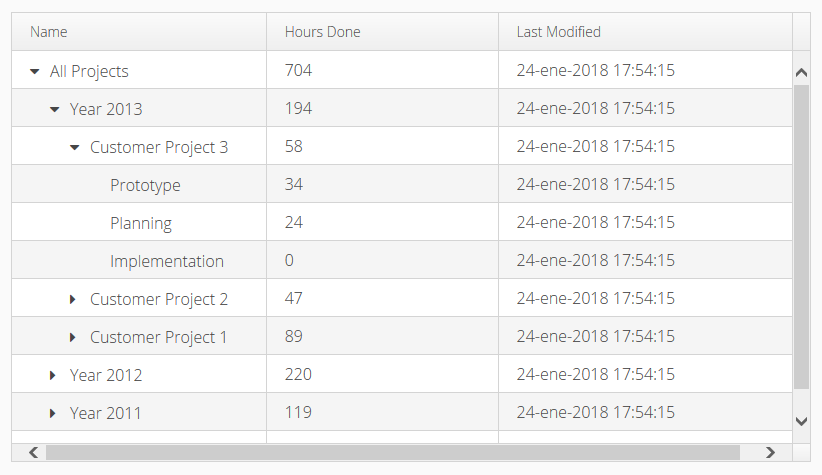
\includegraphics[width=\linewidth]{vaadinExampleImage.png}
	\caption{Árbol de Proyectos}
	\label{fig:vaadinExampleImage}
\end{figure}

A continuación, se explica un ejemplo de contrucción de una jerarquía de tareas propias en la gestión de proyectos por parte de un Jefe de Proyecto (Figura~\ref{fig:vaadinExampleImage}).

El proyecto creado para realizar el ejemplo se compone de una interfaz de usuario (Figura~\ref{fig:uiVaadin}) la cuál utiliza un componente llamado TreeGrid  (será explicado posteriormente,Figura~\ref{fig:treeGrid}) y un contenedor de datos (Figura~\ref{fig:demoContainer}).

Para entrar en contexto con la implementación de un proyecto en Vaadin, es necesario recalcar que el objetivo es abstraer al usuario de todo el comportamiento gráfinco implementado en HTML o Javascript, por lo tanto, para poder crear las estructuras que finalmente desembocarán en elementos gráficos, Vaadin utiliza los llamados componentes.

Un componente es una interfaz de alto nivel, todo elemento gráfico que se quiera utilizar debe de implementar y extender de las clases \emph{Component}\cite{componentVaadin} y \emph{AbstractComponent}\cite{abstractComponentVaadin}, éstas constan de toda la implementación por defecto necesaria para poder mostrar un elemento.

La Figura~\ref{fig:uiVaadin} reprensenta la interfaz gráfica que se ha implementado para el ejemplo. En ella podemos ver que se ha creado un \emph{layout} o espacio reservado en la interfaz para insertar componentes, y se le ha establecido dos características, la primera es un espaciado entre los componentes y la segunda es un márgen sobre los cuatro lados del componente (Figura~\ref{fig:uiVaadin}, Líneas~4-6).

Posteriormente se declara el componente \emph{TreeGrid} que será el encargado de representar la jerarquía de elementos, además, se le ha dado un ancho y alto al elemento de 800 y 450 píxeles respectivamente (Figura~\ref{fig:uiVaadin}, Líneas~8-10).

Para que un componente muestre datos se le debe de insertar un contenedor de datos, en nuestro caso se ha creado una clase que se explicará más adelante que proporciona esta característica, y se le insertado a dicho componente (Figura~\ref{fig:uiVaadin}, Líneas~12-13).

Por último, se ha añadido el componente al \emph{layout} y este al contenido de la interfaz (Figura~\ref{fig:uiVaadin}, Líneas~15-16).

\begin{figure}[!tb]
	\centering
	\begin{lstlisting}[language=Java]
	@Override
	protected void init(VaadinRequest request) {
	
		final VerticalLayout layout = new VerticalLayout();
		layout.setSpacing(true);
		layout.setMargin(true);
		
		final TreeGrid grid = new TreeGrid();
		grid.setWidth(800, Unit.PIXELS);
		grid.setHeight(450, Unit.PIXELS);
		
		DemoContainer container = new DemoContainer();
		grid.setContainerDataSource(container);
		
		layout.addComponent(grid);
		setContent(layout);
	}
	\end{lstlisting}
	\caption{Interfaz de Usuario Vaadin}
	\label{fig:uiVaadin}
\end{figure}

La clase \emph{TreeGrid} es la encargada de mostrar los datos de forma jerárquica. Para cumplimentar esta interfaz, se extiende de la clase de Vaadin \emph{Grid} la cuál permite crear una tabla de forma sencilla con solo implemetar sus métodos. Respecto a la clase \emph{TreeGrid}, con extenderla, ya es capaz de crear una lista jerárquica sobre la tabla. Esta clase posee métodos para añadir y eliminar \emph{listeners} para contraer y expandir el árbol de elementos (Figura~\ref{fig:treeGrid}, Líneas~18-32), para \emph{settear} (Figura~\ref{fig:treeGrid}, Líneas~3-15), y el método para ver desde fuera el estado del componente (Figura~\ref{fig:treeGrid}, Líneas~35-38). El estado del \emph{TreeGrid} es una clase que contiene el identificador de la columna que está siendo modificada por el usuario (Figura~\ref{fig:treeGridState}).


\begin{figure}[!tb]
	\centering
	\begin{lstlisting}[language=Java]
	public class TreeGrid extends Grid {
		
		@Override
		public void setContainerDataSource(Container.Indexed container) {
			if (container != null) {
				if (!(container instanceof Container.Hierarchical)) {
					container = new IndexedContainerHierarchicalWrapper(container);
				}
				
				if (!(container instanceof Collapsible)) {
					container = new ContainerCollapsibleWrapper(container);
				}
			}
			super.setContainerDataSource(container);
		}
		
		
		public void addExpandListener(ExpandEvent.ExpandListener listener) {
			addListener(ExpandEvent.class, listener, ExpandEvent.ExpandListener.EXPAND_METHOD);
		}
		
		public void removeExpandListener(ExpandEvent.ExpandListener listener) {
			removeListener(ExpandEvent.class, listener, ExpandEvent.ExpandListener.EXPAND_METHOD);
		}
		
		public void addCollapseListener(CollapseEvent.CollapseListener listener) {
			addListener(CollapseEvent.class, listener, CollapseEvent.CollapseListener.COLLAPSE_METHOD);
		}
		
		public void removeCollapseListener(CollapseEvent.CollapseListener listener) {
			removeListener(CollapseEvent.class, listener, CollapseEvent.CollapseListener.COLLAPSE_METHOD);
		}
		
		
		@Override
		protected TreeGridState getState() {
			return (TreeGridState) super.getState();
		}
	}
	\end{lstlisting}
	\caption{Componente TreeGrid}
	\label{fig:treeGrid}
\end{figure}

\begin{figure}[!tb]
	\centering
	\begin{lstlisting}[language=Java]
	public class TreeGridState extends GridState {
		public String hierarchyColumnId;
	}
	\end{lstlisting}
	\caption{Componente TreeGrid}
	\label{fig:treeGridState}
\end{figure}


La última clase para explicar es \emph{DemoContainer}  (Figura~\ref{fig:demoContainer}), esta clase extiende de una clase de Vaadin llamada \emph{HierarchicalContainer} que se encarga de realizar toda la lógica para expandir y contraer los nodos, además, implementa las clases de Vaadin \emph{Collapsible} (Figura~\ref{fig:demoContainerCollapsible}) y \emph{Measurable} (Figura~\ref{fig:demoContainerMeasurable}), encargadas de colapsar el árbol de elementos y de calcular la profundidad del elemento en la jerarquía respectivamente.




\begin{figure}[!tb]
	\centering
	\begin{lstlisting}[language=Java]
	public class DemoContainer extends HierarchicalContainer implements Collapsible, Measurable {
	
		static final String PROPERTY_NAME = "Name";
		static final String PROPERTY_HOURS = "Hours done";
		static final String PROPERTY_MODIFIED = "Last modified";
		
		public DemoContainer() {
			addContainerProperty(PROPERTY_NAME, String.class, "");
			addContainerProperty(PROPERTY_HOURS, Integer.class, 0);
			addContainerProperty(PROPERTY_MODIFIED, Date.class, new Date());
			
			for (Object[] r : DataSource.getRoot()) {
				addItem(r);
			}
			
			setItemSorter(new DemoItemSorter());
		}
		
		private Object addItem(Object[] values) {
			Item item = addItem((Object) values);
			setProperties(item, values);
			return values;
		}
		
		private Object addChild(Object[] values, Object parentId) {
			Item item = addItemAfter(parentId, values);
			setProperties(item, values);
			setParent(values, parentId);
			return values;
		}
		
		private void setProperties(Item item, Object[] values) {
			item.getItemProperty(PROPERTY_NAME).setValue(values[0]);
			item.getItemProperty(PROPERTY_HOURS).setValue(values[1]);
			item.getItemProperty(PROPERTY_MODIFIED).setValue(values[2]);
		}

		private void addChildren(Object itemId) {
			for (Object[] child : DataSource.getChildren(itemId)) {
				Object childId = addChild(child, itemId);
				if (Boolean.TRUE.equals(expandedNodes.get(childId))) {
					addChildren(childId);
				}
			}
		}
		
		private boolean removeChildrenRecursively(Object itemId) {
			boolean success = true;
			Collection<?> children2 = getChildren(itemId);
			if (children2 != null) {
				Object[] array = children2.toArray();
				for (int i = 0; i < array.length; i++) {
					boolean removeItemRecursively = removeItemRecursively(
					this, array[i]);
					if (!removeItemRecursively) {
						success = false;
					}
				}
			}
			return success;	
		}
		
		@Override
		public boolean hasChildren(Object itemId) {
			return !DataSource.isLeaf(itemId);
		}
		
	}
	\end{lstlisting}
	\caption{Contenedor TreeGrid}
	\label{fig:demoContainer}
\end{figure}


\begin{figure}[!tb]
	\centering
	\begin{lstlisting}[language=Java]
	public class DemoContainer
	
		...
	
		private Map<Object, Boolean> expandedNodes = new HashMap<>();
			
		@Override
		public void setCollapsed(Object itemId, boolean collapsed) {
			expandedNodes.put(itemId, !collapsed);	
			if (collapsed) {
				removeChildrenRecursively(itemId);
			} else {
				addChildren(itemId);
			}
		}
		
		@Override
		public boolean isCollapsed(Object itemId) {
			return !Boolean.TRUE.equals(expandedNodes.get(itemId));
		}
	}
	\end{lstlisting}
	\caption{Contenedor TreeGrid Collapsible}
	\label{fig:demoContainerCollapsible}
\end{figure}

\begin{figure}[!tb]
	\centering
	\begin{lstlisting}[language=Java]	
	public class DemoContainer
	
		...
		@Override
		public int getDepth(Object itemId) {
			int depth = 0;
			while (!isRoot(itemId)) {
				depth ++;
				itemId = getParent(itemId);
			}
			return depth;
		}
	}
	\end{lstlisting}
	\caption{Contenedor TreeGrid Measurable}
	\label{fig:demoContainerMeasurable}
\end{figure}


Con estas indicaciones se ha creado un ejemplo sencillo de composición de elementos jerárquicos entre sí utilizando Vaadin, como podemos ver ha facilitado mucho su implementación respecto a una configuración basada en \emph{HTML} o \emph{Javascript}.


 			
\section{Arquitectura LUCA}

\input{antecedentes/arquitecturaLUCA.tex}	

\section{Sumario}

El presente capítulo ha presentado todos los conceptos y tecnologías necesarias para poder comprender el trabajo presentado en esta memoria. En primer lugar se ha introducido el framework GoJS, que es el que se ha utilizado para implementar el editor gráfico para la especificación de consultas concatenadas o procesos dentro de LUCA. Dado que este proyecto se integra dentro de la herramienta LUCA, se ha descrito la arquitectura de la misma, para lo que ha sido necesario introducir el patrón \emph{Modelo-Vista-Presentador} y \emph{Vaadin}, por ser esta la tecnología sobre la que se sustenta la herramienta LUCA.  

	
	

	
	
	
	\clearpage
	
	\chapter{Process-Component}
	
	

Este fragmento del proyecto se dedica exclusivamente al apartado gráfico.Es una herramienta que se dedica a proveer métodos para interactuar con él, y además, es capaz mediante \emph{listeners} de avisar a los clientes que lo requieran sobre los eventos ocurridos sobre la interfaz gráfica.


Su implementación se centra en dos pilares. Por una parte se ha realizado un proyecto Vaadin encargado de mantener el estado de la aplicación gráfica, y por otro lado un conjunto de ficheros Javascript implementados sobre GO.JS que se encargan de modificar el entorno gráfico mediante sentencias .
\begin{itemize}
	\item Proyecto Vaadin
	\subitem Este proyecto es el encargado de crear los metodos necesarios para interactuar desde el exterior con el esquema creado previamente. Además debe de permitir insertar \emph{listeners} para los eventos proporcionados desde GO.JS, de forma que se pueda establecer dos direcciones de comunicación. Una desde el exterior con el proyecto Vaadin y este con el conector y directamente con el entorno gráfico de GO.JS, y otro desde interacción con los eventos (por parte del usuario) desde el fichero Javascript de configuración, con el conector y este con el estado, es decir, con el proyecto Vaadin.
	
	\item Ficheros Javascript
	\subitem Existe un primer fichero que permite configurar el esquema gráfico que se va a llevar a cabo (Procesos, Subprocesos, InputVariables, OutputVariables ...), así como todo el resto de propiedades gráficas, además de ser capaz de lanzar eventos preconfigurados.
	
	
	El segundo fichero esencial para el funcionamiento de esta estructura, es el fichero conector. Este es el encargado de declarar y configurar todos los eventos que se pueden lanzar, además de ser el encargado de realizar todos los metodos CRUD \footnote{CRUD es el acrónimo de crear, leer, actualizar y borrar, en esete contexto significa el conjunto de métodos para poder realizar dichas acciones sobre los distintos elementos existentes.}necesarios para que puedan interactuar con las propiedades configuradas en el primer fichero citado previamente.
\end{itemize}


\subsection{Ejemplo Vaadin + Javascript}

El primer paso para comprender el funcionamiento de \emph{Vaadin} es entender su arquitectura básica. Como podemos observar en la Figura~\ref{fig:schema}, consta de tres módulos bien diferenciados. El primer módulo se corresponde con el proyecto implementado en Java. El segundo con el conector en javascript que servirá de comunicador o intermediario entre la librería Javascript y el proyecto. El último se corresponde con la librería Javascript, un ejemplo de esta es GoJS, explicada previamente, por lo tanto, no se mencionará más de ella más allá de que es la encargada del entorno gráfico.



\begin{figure}[!tb]
	\centering
	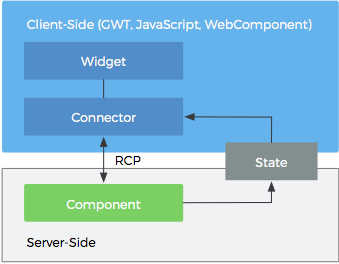
\includegraphics[width=\linewidth]{schema.png}
	\caption{Interacción Vaadin}\label{fig:schema}
\end{figure}




En este proyecto la pieza central que será la encargada de comunicarse con el conector será un componente abstracto que implementa \emph{Vaadin} para llevar a cabo esta finalidad.

Este componente consta de dos partes, por un lado tiene una clase que extiende de \emph{AbstractJavaScriptComponent} (Figura~\ref{fig:componenteVaadin}~,~Línea 2) que será la pieza que posea el contexto para comunicarse con el conector, además, en esta parte se especificarán todos los ficheros Javascript u hojas de estilo que sean necesarios (Figura~\ref{fig:componenteVaadin}~,~Línea 1). Por otro lado el estado de dicho componente, que se encargará de asegurar la integridad de los elementos que existen dentro del componente y extenderá de \emph{JavaScriptComponentState} (Figura~\ref{fig:estadoComponenteVaadin}~,~Línea 1).

\begin{figure}[!tb]
	\centering
	\begin{lstlisting}[language=Java]
	@JavaScript({ "connector.js" })
	public class Component extends AbstractJavaScriptComponent {
		public Component(String content) {
			getState().content = content;
		}
		
		@Override
		protected ComponentState getState() {
			return (ComponentState) super.getState();
		}
	}\end{lstlisting}
	\caption{Componente Vaadin}
	\label{fig:componenteVaadin}
\end{figure}


\begin{figure}[!tb]
	\centering
	\begin{lstlisting}[language=Java]
	public class ComponentState	extends JavaScriptComponentState {
		public String content;
	}\end{lstlisting}
	\caption{Estado Componente Vaadin}
	\label{fig:estadoComponenteVaadin}
\end{figure}


La comunicación del componente con el conector se puede realizar de varias formas, las más comunes son:
\begin{itemize}
	\item  Cambiando el estado del componente, ya que se ejecutará automáticamente una llamada en el conector por dicho cambio(Figura~\ref{fig:conectorDesc}~,~Líneas 6-8).
	\item  Haciendo una llamada al conector mediante una función previamente publicada (Figura~\ref{fig:callfunction}~,~Línea 1). De esta forma se puede elegir la función a la que llamar pasando una serie de parámetros.
\end{itemize}

\begin{figure}[!tb]
	\centering
	\begin{lstlisting}[language=JavaScript]
	callFunction("updateState",content);
	\end{lstlisting}
	\caption{Llamada al conector}
	\label{fig:callfunction}
\end{figure}



\subsubsection{Javascript Connector}	


El conector es el encargado de comunicarse con ambos lados, es decir, con el proyecto Java y el framework Javascript.

Se empieza con la declaración de la localización del conector bajo la nomenclatura \emph{window+dirección+nombre del conector}, y después se especifica el conector (Figura~\ref{fig:conectorDesc}~,~Línea 1).

El conector se compone principalmente de una función que se ejecuta cuando el estado del Componente en Vaadin cambia (Figura~\ref{fig:conectorDesc}~,~Líneas~4-6). Además, se le pueden añadir todas las funciones necesarias para el correcto funcionamiento (Figura~\ref{fig:conectorDesc}~,~Líneas~8-10). Como se puede observar en la Figura~\ref{fig:conectorDesc}~,~Línea~3, se crea un componente, este componente se correspondería, aplicando el caso al que se utilizará posteriormente en el proyecto, a \emph{GoJS}.


\begin{figure}[!tb]
	\centering
	\begin{lstlisting}[language=JavaScript]
	window.urlPaquete_connector = function() {
	
		var mycomponent = 
		new mylibrary.MyComponent(this.getElement());
		
		this.onStateChange = function() {
			mycomponent.content = this.getState().content;
		}
		
		this.updateState = function(content){
			mycomponent.content = content;
		}
	}\end{lstlisting}
	\caption{Conector}
	\label{fig:conectorDesc}
\end{figure}

En conclusión, se ha explicado un ejemplo de interacción del componente Vaadin con un Framework Javascript a través de un conector Javascript.
	
	\clearpage
	
	\chapter{Luca-Process}
	
Este capitulo describe el proceso de desarrollo e integración del componente gráfico (Process-Component). Se analizarán los aspectos del diseño y arquitectura a realizar así como las etapas de desarrollo del mismo.
	
\section{Arquitectura}

La arquitectura  de Luca-Process tras la integración del Process-Component, cambia ligera o mínimamente respecto a la arquitectura demostrada en la introducción. La siguiente figura describe la diferencia respecto a la figura anterior:

\begin{figure}[H]
	\centering
	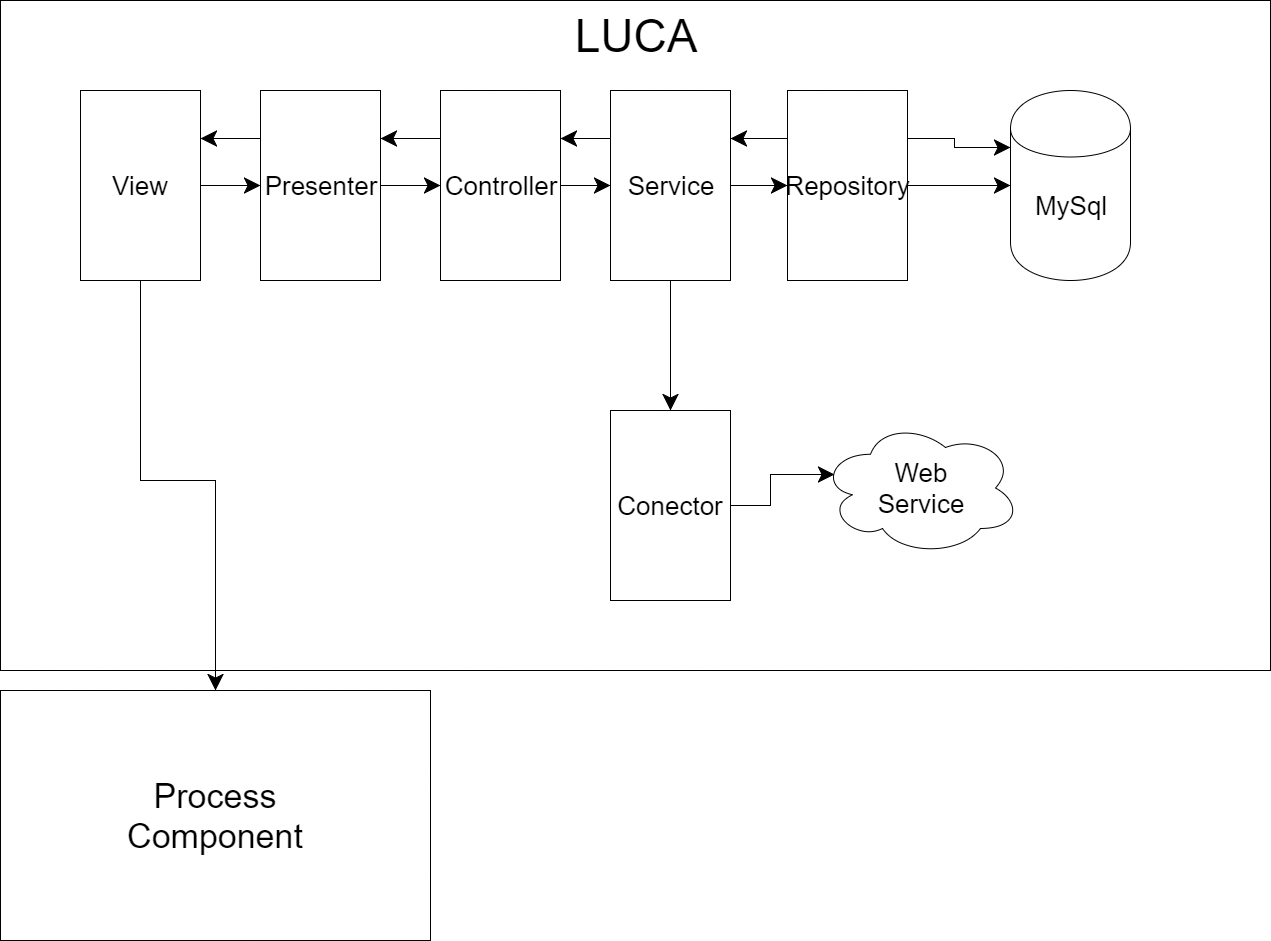
\includegraphics[scale=0.5]{arquitecturaLuca.png}
	\caption{Nueva Arquitectura de LUCA}\label{fig:arquitecturaLuca}
\end{figure}

Como se puede apreciar, la única diferencia reside en que en esta citada nueva funcionalidad se utiliza otro proyecto aparte, el cuál se encarga de forma exclusiva de proveer componentes de visualización para poder abordar la sintaxis de procesos y subprocesos que se enlazan entre sí mediante entradas y salidas.

\section{Desarrollo}

En esta sección se describe el proceso de desarrollo o implementación del componente de LUCA que integra el componente gráfico.


El primer paso para empezar a comprender el diseño y arquitectura de LUCA, fue realizar una pequeña prueba de concepto aplicando el patrón MVP\cite{mvp} e importando el componente gráfico para mostrar un proceso provisional, comprobando así el comportamiento del componente.



Una vez comprobado el funcionamiento, se comienza la implementación por capas del proyecto, creando la capa controladora junto con sus anotaciones de seguridad, la capa de servicio que realiza llamadas a la capa de repositorio (implementada con Spring Data\cite{jpa}) para acceder a la base de datos, así como, al resto de servicios ya existentes en LUCA para la obtención de datos y ejecución de consultas. También se realizaron e implementaron, como se citó en la introducción, el conjunto de pruebas sobre la capa de servicio.



Con la solidez de las capas de datos implementadas, se prosiguió con el diseño de la capa de presentación para componer todas las vistas y los presentadores necesarios. Para ello hubo que, siguiendo el diseño preestablecido, diseñar para cada vista principal(aquellas vistas que albergan al resto y que forman una unidad de interacción completa, por ejemplo la vista de gestión de procesos, de creación o de ejecución) un conjunto de vistas de acciones y de una vista de visualización de datos, cada una implementada con una pareja de vista presentador.


Finalmente, tras realizar la implementación de componente, se realizó un comprobación y satisfacción de los requisitos generales descritos en la introducción.



	
	\clearpage
	
	\chapter{Sumario, Conclusiones y Trabajos Futuros}

\section{Sumario}

El presente documento ha descrito el trabajo realizado para integrar el concepto de \emph{proceso} en LUCA. Gracias a este trabajo es posible ejecutar en LUCA procesos de recuperación de la información que requieran de la ejecución de varias consultas encadenadas, donde las salidas de ciertas consults sirvan como entradas de otras. 

Dado que el trabajo presentado se enmarca dentro del proyecto LUCA, en primer lugar se ha descrito dicho proyecto en profundidad; detallando su objetivo, que es el de proporcionar mecanismos de acceso uniforme a fuentes de datos heterogéneas, y sus limitaciones. Entre dichas limitaciones se encontraba la carencia de un soporte adecuado para ejecutar procesos de recuperación de la información que precisasen de la ejecución de varias consultadas encadenadas. Antes del desarrollo del proyecto, el usuario debía ejecutar cada consulta del conjunto de consultas encadenadas manualmente, guardar sus resultados y manipularlos adecuadamente para posteriormente poder usarlos como entradas para otras consultas. 

Para paliar esta deficiencia, los directores de LUCA habían elaborado una especificación de requisitos para un nuevo módulo de LUCA que soportase el concepto de proceso, incluyendo tanto su especificación, la definición del proceso, como su ejecución. Dado que la especificación de requisitos ya estaba hecha, y la arquitectura definida, este proyecto fin de carrera se circunscribe a las fase de diseño detallado, implementación y pruebas. 

Una vez definidas la motivación y el alcance del proyecto, se describieron una serie de tecnologías necesarias para entender su funcionamiento. En primer lugar se explicó el funcionamiento del framework \emph{GoJS} cuyo objetivo es facilitar la creación de editores gráficos en Javascript, el cual fue utilizado en el desarrollo del proyecto para la creación del editor gráfico de procesos. A continuación, se describió la arquitectura de LUCA, que es el proyecto raíz donde se integra el módulo desarrollado en este Trabajo Fin de Grado. Dado que LUCA está construido sobre \emph{Vaadin}, un framework para el desarrollo de aplicaciones web enriquecidas desde código Java, y que \emph{Vaadin} sigue el patrón \emph{Model-View-Presenter}, antes de describir la arquitectura de LUCA se introdujeron ambos elementos. 

Finalmente, se describieron las diversas fases del desarrollo del presente proyecto. El proyecto se ha desarrollado de manera iterativa, moviéndonos en cada iteración desde la capa de presentación a la capa de persistencia. 

\section{Resultados}

Gracias a este proyecto, LUCA soporta actualmente el concepto de \emph{proceso}. Más concretamente, gracias a este proyecto, LUCA soporta ahora las siguientes funcionalidades. 

\begin{enumerate}
	\item Especificación gráfica de \emph{procesos}, mediante la definición de las consultas que componen dicho proceso y su interconexión.
	\item Alteración de la ejecución del flujo de ejecución de un proceso en función de los valores de las salidas.
    \item Comprobación de la corrección de la conexión entre salidas y entradas de las consultas que componen un proceso.
    \item Ejecución de procesos.
	\item Ejecución paso a paso de los procesos.
	\item Exportar los resultados de los procesos.
\end{enumerate}

\section{Conclusiones}

%% Detalla qué conocimientos del Grado te han sido especialmente útiles.

La experiencia durante el desarrollo del proyecto ha sido más que satisfactoria, ya que los conocimientos que he aprendido a lo largo del grado, tales como los patrones de diseño, las diferentes arquitecturas software o el despliegue de servicios entre muchos otros , han sido indispensables para poder llevarlo a cabo. Además, debido al uso de nuevos frameworks y herramientas, he sido capaz de ampliar mis conocimientos, a los que he incorporado la utilización de frameworks como \emph{Vaadin} y \emph{GoJS}.

La oportunidad de llevar a cabo el proyecto en la empresa CIC Consulting Informático, me ha permitido adquirir un hábito de trabajo, así como de responsabilidades y fijaciones a horarios que no se puede aprender de ninguna otra forma. Además, el apoyo recibido por el equipo de LUCA ha sido excepcional y he podido aprender mucho con ellos.

\section{Trabajos Futuros}

Con el proyecto integrado en LUCA, se espera poder realizar el trabajo realizado en futuras versiones del producto. Concretamente, se plantea la posibilidad de soportar procesos anidados, es decir, la capacidad de utilizar procesos ya definidos como si fuesen consultas simples para la definición de un nuevo proceso. Es decir, permitir que los procesos puedan contener procesos. También se plantea la posibilidad de crear consultas desde una consola gráfica, utilizando el editor gráfico, ya que en algunos casos este estilo de especificación puede resultar más conveniente.


		
	
	\clearpage

	


	
	\bibliographystyle{acm}
	\bibliography{Bibliografia}
	

\end{document}


